\documentclass[12pt]{article}
\usepackage[english]{babel}
\usepackage{natbib}
\usepackage{url}
\usepackage[utf8x]{inputenc}
\usepackage{amsmath}
\usepackage{amsfonts}
\usepackage{color}
\usepackage{listings}
\definecolor{cadetgrey}{rgb}{0.57, 0.64, 0.69}
\usepackage{graphicx}
\graphicspath{{images/}}
\usepackage{parskip}
\usepackage{fancyhdr}
\usepackage{vmargin}
\setmarginsrb{3 cm}{2.5 cm}{3 cm}{2.5 cm}{1 cm}{1.5 cm}{1 cm}{1.5 cm}
\lstdefinelanguage{JavaScript}{
      morekeywords={break, case, catch, continue, debugger, default, delete, do, else, false, finally, for, function, if, in, instanceof, new, null, return, switch, this, throw, true, try, typeof, var, void, while, with},
      morecomment=[s]{/*}{*/},
      morecomment=[l]//,
      morestring=[b]",
      morestring=[b]'
    }
\lstdefinelanguage{CSS}{
 language=css,
      keywords={accelerator,azimuth,background,background-attachment,
            background-color,background-image,background-position,
            background-position-x,background-position-y,background-repeat,
            behavior,border,border-bottom,border-bottom-color,
            border-bottom-style,border-bottom-width,border-collapse,
            border-color,border-left,border-left-color,border-left-style,
            border-left-width,border-right,border-right-color,
            border-right-style,border-right-width,border-spacing,
            border-style,border-top,border-top-color,border-top-style,
            border-top-width,border-width,bottom,caption-side,clear,
            clip,color,content,counter-increment,counter-reset,cue,
            cue-after,cue-before,cursor,direction,display,elevation,
            empty-cells,filter,float,font,font-family,font-size,
            font-size-adjust,font-stretch,font-style,font-variant,
            font-weight,height,ime-mode,include-source,
            layer-background-color,layer-background-image,layout-flow,
            layout-grid,layout-grid-char,layout-grid-char-spacing,
            layout-grid-line,layout-grid-mode,layout-grid-type,left,
            letter-spacing,line-break,line-height,list-style,
            list-style-image,list-style-position,list-style-type,margin,
            margin-bottom,margin-left,margin-right,margin-top,
            marker-offset,marks,max-height,max-width,min-height,
            min-width,-moz-binding,-moz-border-radius,
            -moz-border-radius-topleft,-moz-border-radius-topright,
            -moz-border-radius-bottomright,-moz-border-radius-bottomleft,
            -moz-border-top-colors,-moz-border-right-colors,
            -moz-border-bottom-colors,-moz-border-left-colors,-moz-opacity,
            -moz-outline,-moz-outline-color,-moz-outline-style,
            -moz-outline-width,-moz-user-focus,-moz-user-input,
            -moz-user-modify,-moz-user-select,orphans,outline,
            outline-color,outline-style,outline-width,overflow,
            overflow-X,overflow-Y,padding,padding-bottom,padding-left,
            padding-right,padding-top,page,page-break-after,
            page-break-before,page-break-inside,pause,pause-after,
            pause-before,pitch,pitch-range,play-during,position,quotes,
            -replace,richness,right,ruby-align,ruby-overhang,
            ruby-position,-set-link-source,size,speak,speak-header,
            speak-numeral,speak-punctuation,speech-rate,stress,
            scrollbar-arrow-color,scrollbar-base-color,
            scrollbar-dark-shadow-color,scrollbar-face-color,
            scrollbar-highlight-color,scrollbar-shadow-color,
            scrollbar-3d-light-color,scrollbar-track-color,table-layout,
            text-align,text-align-last,text-decoration,text-indent,
            text-justify,text-overflow,text-shadow,text-transform,
            text-autospace,text-kashida-space,text-underline-position,top,
            unicode-bidi,-use-link-source,vertical-align,visibility,
            voice-family,volume,white-space,widows,width,word-break,
            word-spacing,word-wrap,writing-mode,z-index,zoom},
      sensitive=true,
      morecomment=[l]{//},
      morecomment=[s]{/*}{*/},
      morestring=[b]',
      morestring=[b]",
      alsoletter={:},
      alsodigit={-}
    }
 \lstdefinelanguage{HTML5}{
            language=html,
            sensitive=true, 
            alsoletter={<>=-},
            otherkeywords={
            % HTML tags
            <, </, >,
            </a, <a, </a>,
            </abbr, <abbr, </abbr>,
            </address, <address, </address>,
            </area, <area, </area>,
            </area, <area, </area>,
            </article, <article, </article>,
            </aside, <aside, </aside>,
            </audio, <audio, </audio>,
            </audio, <audio, </audio>,
            </b, <b, </b>,
            </base, <base, </base>,
            </bdi, <bdi, </bdi>,
            </bdo, <bdo, </bdo>,
            </blockquote, <blockquote, </blockquote>,
            </body, <body, </body>,
            </br, <br, </br>,
            </button, <button, </button>,
            </canvas, <canvas, </canvas>,
            </caption, <caption, </caption>,
            </cite, <cite, </cite>,
            </code, <code, </code>,
            </col, <col, </col>,
            </colgroup, <colgroup, </colgroup>,
            </data, <data, </data>,
            </datalist, <datalist, </datalist>,
            </dd, <dd, </dd>,
            </del, <del, </del>,
            </details, <details, </details>,
            </dfn, <dfn, </dfn>,
            </div, <div, </div>,
            </dl, <dl, </dl>,
            </dt, <dt, </dt>,
            </em, <em, </em>,
            </embed, <embed, </embed>,
            </fieldset, <fieldset, </fieldset>,
            </figcaption, <figcaption, </figcaption>,
            </figure, <figure, </figure>,
            </footer, <footer, </footer>,
            </form, <form, </form>,
            </h1, <h1, </h1>,
            </h2, <h2, </h2>,
            </h3, <h3, </h3>,
            </h4, <h4, </h4>,
            </h5, <h5, </h5>,
            </h6, <h6, </h6>,
            </head, <head, </head>,
            </header, <header, </header>,
            </hr, <hr, </hr>,
            </html, <html, </html>,
            </i, <i, </i>,
            </iframe, <iframe, </iframe>,
            </img, <img, </img>,
            </input, <input, </input>,
            </ins, <ins, </ins>,
            </kbd, <kbd, </kbd>,
            </keygen, <keygen, </keygen>,
            </label, <label, </label>,
            </legend, <legend, </legend>,
            </li, <li, </li>,
            </link, <link, </link>,
            </main, <main, </main>,
            </map, <map, </map>,
            </mark, <mark, </mark>,
            </math, <math, </math>,
            </menu, <menu, </menu>,
            </menuitem, <menuitem, </menuitem>,
            </meta, <meta, </meta>,
            </meter, <meter, </meter>,
            </nav, <nav, </nav>,
            </noscript, <noscript, </noscript>,
            </object, <object, </object>,
            </ol, <ol, </ol>,
            </optgroup, <optgroup, </optgroup>,
            </option, <option, </option>,
            </output, <output, </output>,
            </p, <p, </p>,
            </param, <param, </param>,
            </pre, <pre, </pre>,
            </progress, <progress, </progress>,
            </q, <q, </q>,
            </rp, <rp, </rp>,
            </rt, <rt, </rt>,
            </ruby, <ruby, </ruby>,
            </s, <s, </s>,
            </samp, <samp, </samp>,
            </script, <script, </script>,
            </section, <section, </section>,
            </select, <select, </select>,
            </small, <small, </small>,
            </source, <source, </source>,
            </span, <span, </span>,
            </strong, <strong, </strong>,
            </style, <style, </style>,
            </summary, <summary, </summary>,
            </sup, <sup, </sup>,
            </svg, <svg, </svg>,
            </table, <table, </table>,
            </tbody, <tbody, </tbody>,
            </td, <td, </td>,
            </template, <template, </template>,
            </textarea, <textarea, </textarea>,
            </tfoot, <tfoot, </tfoot>,
            </th, <th, </th>,
            </thead, <thead, </thead>,
            </time, <time, </time>,
            </title, <title, </title>,
            </tr, <tr, </tr>,
            </track, <track, </track>,
            </u, <u, </u>,
            </ul, <ul, </ul>,
            </var, <var, </var>,
            </video, <video, </video>,
            </wbr, <wbr, </wbr>,
            />, <!
            },  
            ndkeywords={
            % General
            =,
            % HTML attributes
            accept=, accept-charset=, accesskey=, action=, align=, alt=, async=, autocomplete=, autofocus=, autoplay=, autosave=, bgcolor=, border=, buffered=, challenge=, charset=, checked=, cite=, class=, code=, codebase=, color=, cols=, colspan=, content=, contenteditable=, contextmenu=, controls=, coords=, data=, datetime=, default=, defer=, dir=, dirname=, disabled=, download=, draggable=, dropzone=, enctype=, for=, form=, formaction=, headers=, height=, hidden=, high=, href=, hreflang=, http-equiv=, icon=, id=, ismap=, itemprop=, keytype=, kind=, label=, lang=, language=, list=, loop=, low=, manifest=, max=, maxlength=, media=, method=, min=, multiple=, name=, novalidate=, open=, optimum=, pattern=, ping=, placeholder=, poster=, preload=, pubdate=, radiogroup=, readonly=, rel=, required=, reversed=, rows=, rowspan=, sandbox=, scope=, scoped=, seamless=, selected=, shape=, size=, sizes=, span=, spellcheck=, src=, srcdoc=, srclang=, start=, step=, style=, summary=, tabindex=, target=, title=, type=, usemap=, value=, width=, wrap=,
            % CSS properties
            accelerator:,azimuth:,background:,background-attachment:,
            background-color:,background-image:,background-position:,
            background-position-x:,background-position-y:,background-repeat:,
            behavior:,border:,border-bottom:,border-bottom-color:,
            border-bottom-style:,border-bottom-width:,border-collapse:,
            border-color:,border-left:,border-left-color:,border-left-style:,
            border-left-width:,border-right:,border-right-color:,
            border-right-style:,border-right-width:,border-spacing:,
            border-style:,border-top:,border-top-color:,border-top-style:,
            border-top-width:,border-width:,bottom:,caption-side:,clear:,
            clip:,color:,content:,counter-increment:,counter-reset:,cue:,
            cue-after:,cue-before:,cursor:,direction:,display:,elevation:,
            empty-cells:,filter:,float:,font:,font-family:,font-size:,
            font-size-adjust:,font-stretch:,font-style:,font-variant:,
            font-weight:,height:,ime-mode:,include-source:,
            layer-background-color:,layer-background-image:,layout-flow:,
            layout-grid:,layout-grid-char:,layout-grid-char-spacing:,
            layout-grid-line:,layout-grid-mode:,layout-grid-type:,left:,
            letter-spacing:,line-break:,line-height:,list-style:,
            list-style-image:,list-style-position:,list-style-type:,margin:,
            margin-bottom:,margin-left:,margin-right:,margin-top:,
            marker-offset:,marks:,max-height:,max-width:,min-height:,
            min-width:,transition-duration:,transition-property:,
            transition-timing-function:,transform:,
            -moz-transform:,-moz-binding:,-moz-border-radius:,
            -moz-border-radius-topleft:,-moz-border-radius-topright:,
            -moz-border-radius-bottomright:,-moz-border-radius-bottomleft:,
            -moz-border-top-colors:,-moz-border-right-colors:,
            -moz-border-bottom-colors:,-moz-border-left-colors:,-moz-opacity:,
            -moz-outline:,-moz-outline-color:,-moz-outline-style:,
            -moz-outline-width:,-moz-user-focus:,-moz-user-input:,
            -moz-user-modify:,-moz-user-select:,orphans:,outline:,
            outline-color:,outline-style:,outline-width:,overflow:,
            overflow-X:,overflow-Y:,padding:,padding-bottom:,padding-left:,
            padding-right:,padding-top:,page:,page-break-after:,
            page-break-before:,page-break-inside:,pause:,pause-after:,
            pause-before:,pitch:,pitch-range:,play-during:,position:,quotes:,
            -replace:,richness:,right:,ruby-align:,ruby-overhang:,
            ruby-position:,-set-link-source:,size:,speak:,speak-header:,
            speak-numeral:,speak-punctuation:,speech-rate:,stress:,
            scrollbar-arrow-color:,scrollbar-base-color:,
            scrollbar-dark-shadow-color:,scrollbar-face-color:,
            scrollbar-highlight-color:,scrollbar-shadow-color:,
            scrollbar-3d-light-color:,scrollbar-track-color:,table-layout:,
            text-align:,text-align-last:,text-decoration:,text-indent:,
            text-justify:,text-overflow:,text-shadow:,text-transform:,
            text-autospace:,text-kashida-space:,text-underline-position:,top:,
            unicode-bidi:,-use-link-source:,vertical-align:,visibility:,
            voice-family:,volume:,white-space:,widows:,width:,word-break:,
            word-spacing:,word-wrap:,writing-mode:,z-index:,zoom:
            },  
            morecomment=[s]{<!--}{-->},
            tag=[s]
    }
\lstset{ 
  backgroundcolor=\color{white},   % choose the background color; you must add \usepackage{color} or \usepackage{xcolor}; should come as last argument
  basicstyle=\footnotesize,        % the size of the fonts that are used for the code
  breakatwhitespace=false,         % sets if automatic breaks should only happen at whitespace
  breaklines=true,                 % sets automatic line breaking
  captionpos=b,                    % sets the caption-position to bottom
  %commentstyle=\color{mygreen},    % comment style
  deletekeywords={...},            % if you want to delete keywords from the given language
  escapeinside={\%*}{*)},          % if you want to add LaTeX within your code
  extendedchars=true,              % lets you use non-ASCII characters; for 8-bits encodings only, does not work with UTF-8
  frame=single,	                   % adds a frame around the code
  keepspaces=true,                 % keeps spaces in text, useful for keeping indentation of code (possibly needs columns=flexible)
  keywordstyle=\color{blue},       % keyword style
  language=Python,                 % the language of the code
  morekeywords={*,...},            % if you want to add more keywords to the set
  %numbers=left,                    % where to put the line-numbers; possible values are (none, left, right)
  numbersep=5pt,                   % how far the line-numbers are from the code
  %numberstyle=\tiny\color{mygray}, % the style that is used for the line-numbers
  rulecolor=\color{black},         % if not set, the frame-color may be changed on line-breaks within not-black text (e.g. comments (green here))
  showspaces=false,                % show spaces everywhere adding particular underscores; it overrides 'showstringspaces'
  showstringspaces=false,          % underline spaces within strings only
  showtabs=false,                  % show tabs within strings adding particular underscores
  %stepnumber=2,                    % the step between two line-numbers. If it's 1, each line will be numbered
  %stringstyle=\color{mymauve},     % string literal style
  tabsize=2,	                   % sets default tabsize to 2 spaces
  %title=\lstname                   % show the filename of files included with \lstinputlisting; also try caption instead of title
}

\title{Sino: Haymaking challenge}			% Title
\author{Horpynchenko, Dmytro} 								% Author
\date{\today}											% Date

\makeatletter
\let\thetitle\@title
\let\theauthor\@author
\makeatother

\pagestyle{fancy}
\fancyhf{}

\lhead{\thetitle}
\cfoot{\thepage}

\begin{document}

%%%%%%%%%%%%%%%%%%%%%%%%%%%%%%%%%%%%%%%%%%%%%%%%%%%%%%%%%%%%%%%%%%%%%%%%%%%%%%%%%%%%%%%%%

\begin{titlepage}
	\centering
    
\includegraphics[scale = 0.2]{images/sapienza_logo_only.png}\\[1.0 cm]	% University Logo
    \textsc{\LARGE Sapienza University of Rome}\\[2.0 cm]	% University Name
	\textsc{\Large  }\\[0.5 cm]				% Course Code
	\textsc{\Large Interactive Computer Graphics}\\[0.5 cm]				% Course Name
	\rule{\linewidth}{0.2 mm} \\[0.4 cm]
	{ \huge \bfseries \thetitle}\\
	\rule{\linewidth}{0.2 mm} \\[1.5 cm]

	\begin{minipage}{0.4\textwidth}
		\begin{flushleft} \large
			\emph{Author:}\\
			\theauthor
			\end{flushleft}
			\end{minipage}~
			\begin{minipage}{0.4\textwidth}
			\begin{flushright} \large
			\emph{Student Number:} \\
			1807584				% Your Student Number
		\end{flushright}
	\end{minipage}\\[2 cm]


	\vfill

\end{titlepage}

%%%%%%%%%%%%%%%%%%%%%%%%%%%%%%%%%%%%%%%%%%%%%%%%%%%%%%%%%%%%%%%%%%%%%%%%%%%%%%%%%%%%%%%%%

\tableofcontents
\pagebreak

%%%%%%%%%%%%%%%%%%%%%%%%%%%%%%%%%%%%%%%%%%%%%%%%%%%%%%%%%%%%%%%%%%%%%%%%%%%%%%%%%%%%%%%%%
\section{Intro}
Final project is a browser game with elements of 3D graphics.
%Game must be able to run on following list of browsers 
\subsection{Concept}
The world of the game is a field with hay blocks and obstacles on it. A user is a driver of a vehicle that can move on the field in any direction and collect a hay. In case of collision with the obstacle, vehicle loose all its speed or accelerates in opposite direction in case of high speed. The aim of the game is to collect all hay blocks in defined time period.  Amount of time, hay blocks and obstacles depends on the level of difficulty chosen by user. 
\\
The vehicle has 2 controls available:
\begin{itemize}
\item {
Front wheels steering (left and right) controlled with left and right arrow keys. After release of the keys vehicle's wheels return to their default positions of 0 deg.
}
\item {
Accelerating (forward and backward) using up and down arrow keys accordingly. Release of the keys stop acceleration and leads to deceleration of the vehicle because of the wheel's friction.
}
\end{itemize}
Collecting action is done by colliding with hay block that lead to increase of the score and removing hay item from the field.
\subsection{Name}
The name ``Sino'' comes fron Ukrainian word ``ciho'' - hay \cite{wiki:sino}.

\newpage
\section{Implementation}
\subsection{Overview}
\subsubsection{World}
The world of the game is represented as a simulation of real world with infinite grass field and a blue sky around.

\begin{figure}[h!]
\begin{center}
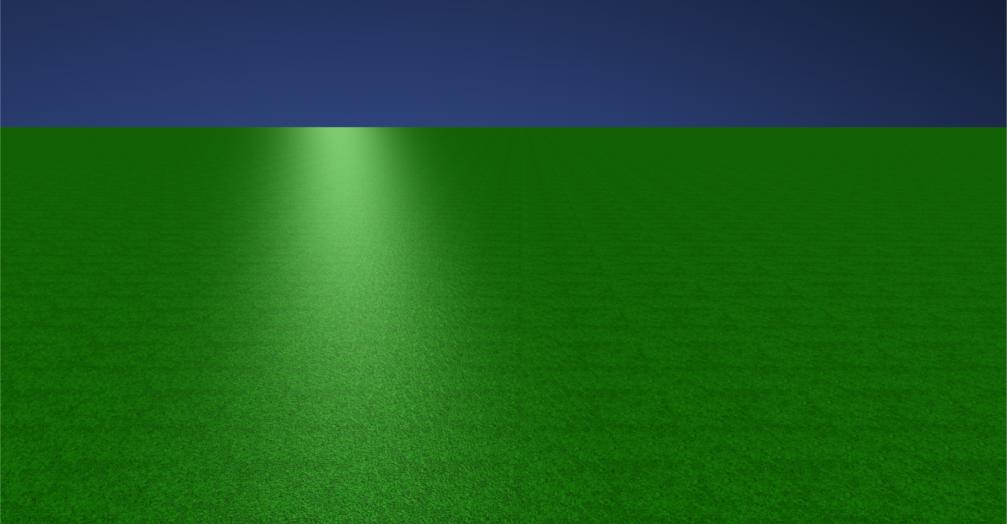
\includegraphics[scale=0.4]{images/env.jpg}
\end{center}
\caption{Game world}
\label{world}
\end{figure}

\subsubsection{Hays and obstacles}
Hays are represented as rectangular cuboid of constant size 1x1x2 with texture of hay (Figure \ref{hay_item}).

\begin{figure}[h!]
\begin{center}
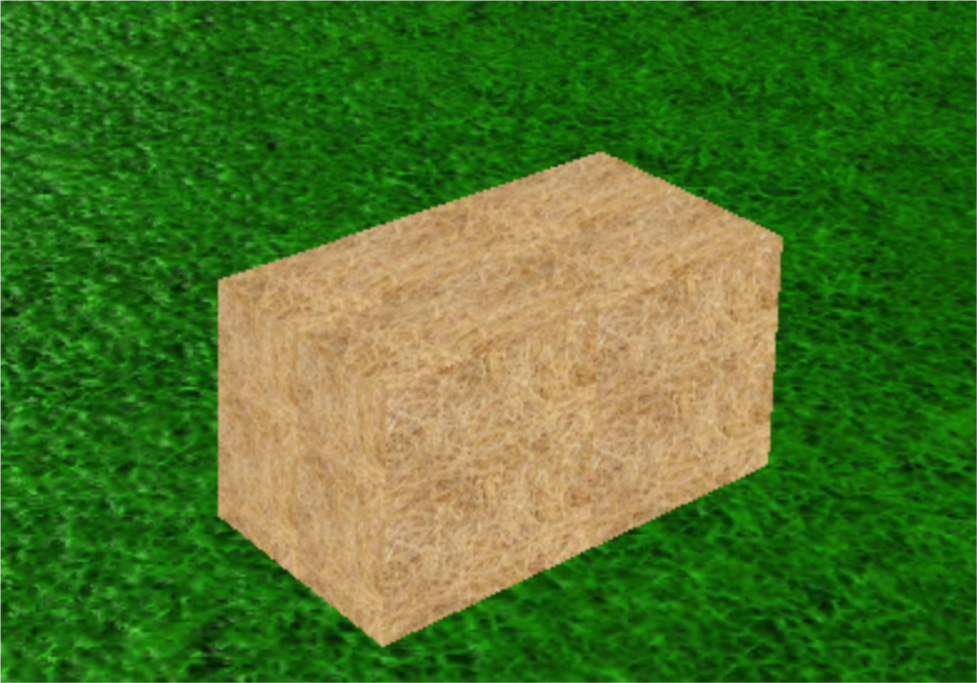
\includegraphics[scale=0.8]{images/hay.png}
\end{center}
\caption{Hay item}
\label{hay_item}
\end{figure}

\par
Obstacles are represented as rectangular cuboid with various sizes. An example of obstacle of size 1x1x4 is showed on Figure \ref{obstacle_item}.

\begin{figure}[h!]
\begin{center}
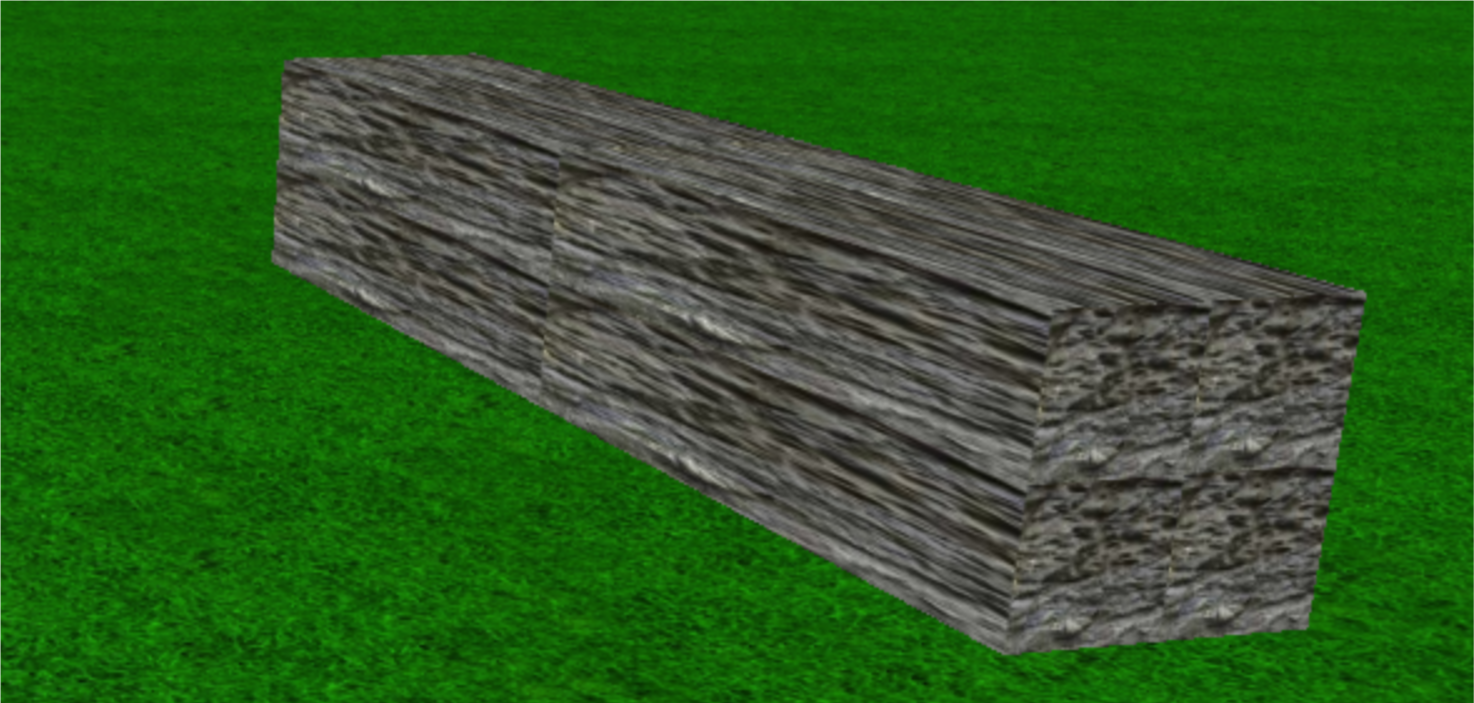
\includegraphics[scale=0.8]{images/obstacle2.png}
\end{center}
\caption{Obstacle item}
\label{obstacle_item}
\end{figure}

\subsubsection{Vehicle}
Vehicle model is a model found on the online marketplace TurboSquid (\url{www.turbosquid.com}). Model represented as tractor vehicle (Figure \ref{tractor1}). For performing an animation 3D model was separated using Blender software into body, front and rear wheels. Every part of the model is exported through Waveform .obj file format for later using during run time. 

\begin{figure}[h!]
\begin{center}
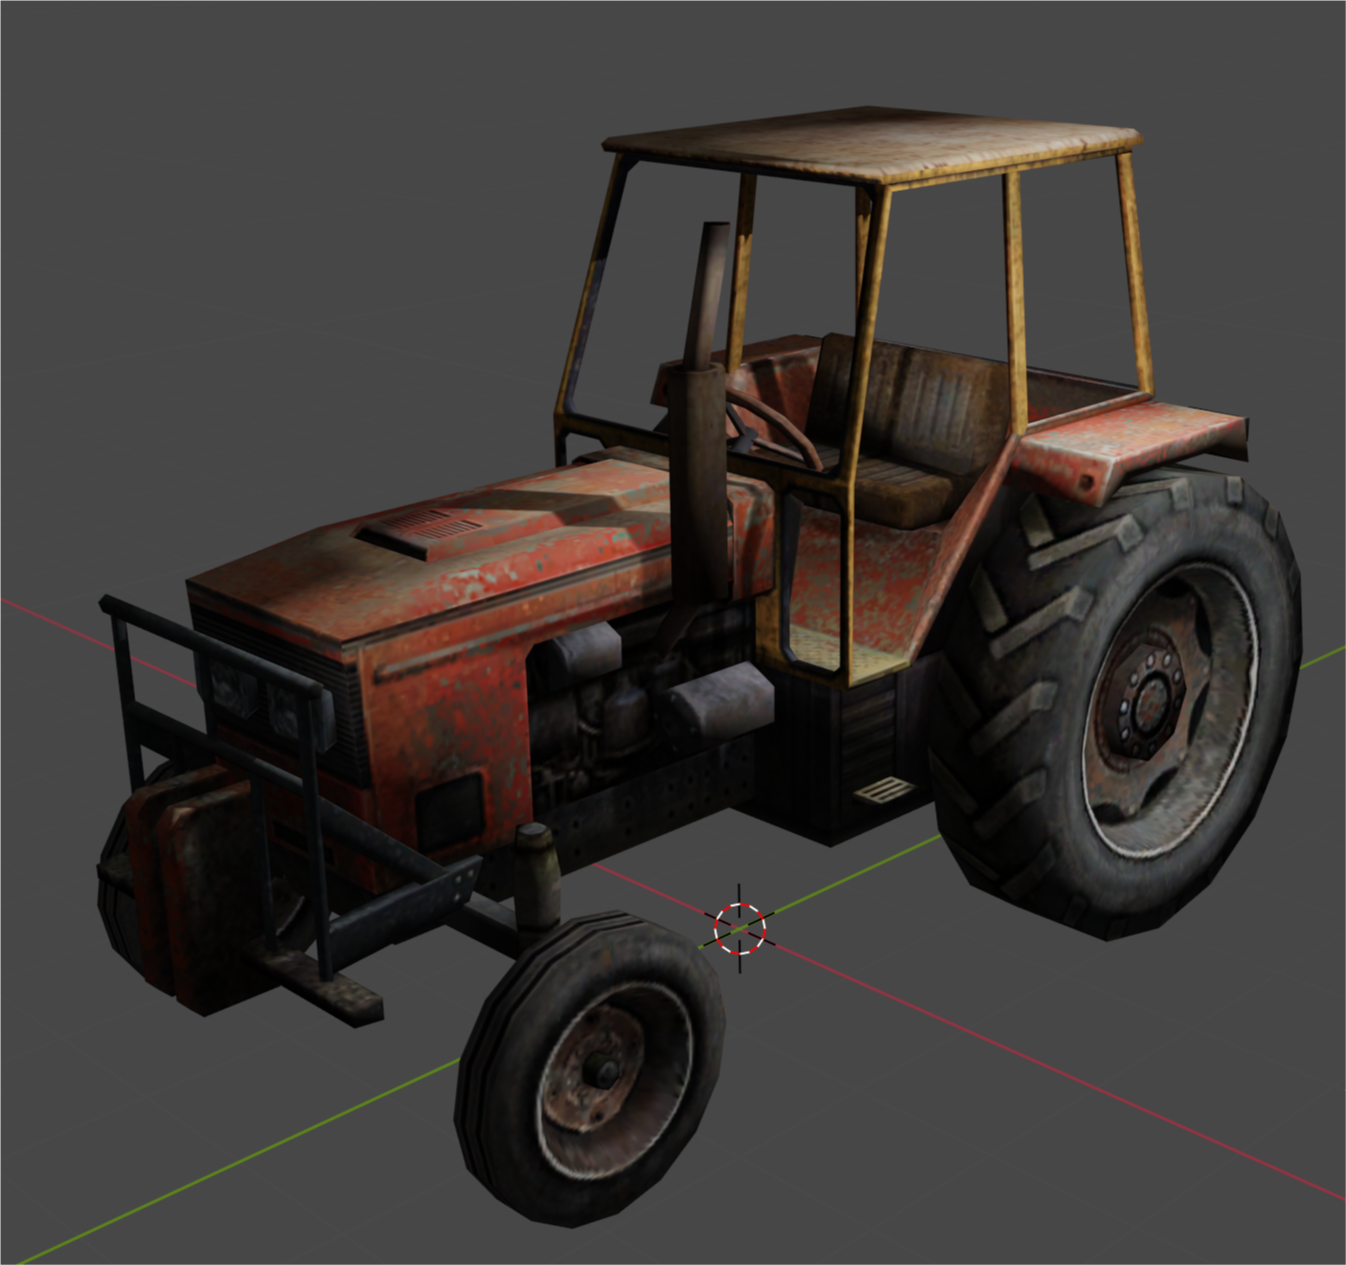
\includegraphics[scale=0.8]{images/tractor_blender.png}
\end{center}
\caption{Tractor model in Blender}
\label{tractor1}
\end{figure}

\subsection{Libraries and Frameworks}
All modern browsers has support of WebGL - a JavaScript API for rendering interactive 2D and 3D graphics with GPU acceleration\citep{wiki:webgl}. But usage of WebGL is quite complicated, requiring writing a lot of boilerplate code, helper functions and hardly maintained code. Thus, in this project THREE.js (\url{https://threejs.org}) open source library was used that offers high-level object-oriented JavaScript API.
\\
Physics emulation libraries like Physi.js or ammo.js weren't used since they are not necessary for game and make big impact on overall performance.
\\
For debug purposes and performance tracking Stats library (\url{https://github.com/mrdoob/stats.js}) is used.
\subsection{HTML}
Hypertext Markup Language (HTML) is the standard markup language for creating web pages and web applications\citep{wiki:html}. Project is represented as a single page web application with \textit{index.html}  as main entrance point and consists of two parts:
\begin{itemize}
\item Head, which includes data, like name of the web page,  author and imports  CSS and JavaScript files.
\item Body that describes structural hierarchy of UI elements on the web page.
\end{itemize}
\subsection{CSS}
CSS (Cascading Style Sheets) is a technology that simplify description and declaration of so called ``styles'' or parameters of elements of HTML page\citep{wiki:css}. ``Sino'' project contains \textit{styles.css} file under css folder that describes parameters of elements of html page. This includes position inside parent, text color and size, paddings and margins, scales etc.
\\
As a font ArcadeClassic was used.
\\
\lstinputlisting[language=html,
%commentstyle=\color{green},
firstline=1, lastline=5,
keywordstyle=\color{blue},
caption={Declaration of custom font}
]
{../css/styles.css}
\subsection{JavaScript}
All algorithm parts are written in JavaScript and consist of few separate js files for easy maintenance.
\subsubsection{game.js}
Entrance point of the game's JavaScript code. Contains game UI initialization, game logic and communication between all other elements of the code.
Includes following functions:
\begin{itemize}
\item \textit{init} - handles creation and setup all components of the program after start.
\item \textit{initScene} - called during init function execution. Initialize and configure main components of THREE.js library renderer and camera.
\item \textit{initUI} - called during init function execution. Initialize sreen UI elements like labels, buttons and their callbacks, Stat library.
\item \textit{addLight} - alled during init function execution. Initialize, configure and add to scene 3 light source: ambient light using lib THREE.js class \textit{AmbientLight} for creating uniform light all along the scene and 2 directional lights from behind and front using class \textit{DirectionalLight}.
\\
\lstinputlisting[language=html,
%commentstyle=\color{green},
firstline=229, lastline=243,
keywordstyle=\color{blue},
caption={Adding light sources}
]
{../js/game.js}

\item \textit{initRendering} - called during init function execution. Describe sequence of operations done for rendering each frame. Call a system function \textit{requestAnimationFrame} to subscribe for next frame update.
\item \textit{onWindowResize} - called during init function execution. Called each time size of the browser window is changed. Adjust renderer and camera output parameters according to new window dimensions.
\\
\lstinputlisting[language=html,
%commentstyle=\color{green},
firstline=197, lastline=203,
keywordstyle=\color{blue},
caption={onWindowResize function}
]
{../js/game.js}

\item \textit{update} - called on every frame update call. Updates vehicle position and configuration, check for vehicle collides with hays and obstacles, update score. Collide check is done using THREE.js \textit{BoundingBox} and it's method \textit{intersectsBox}. In case of intersection of bounding boxes of vehicle and item one is counting as colliding.
\end{itemize}
\subsubsection{core.js}
Contains main components of the game such as:
\begin{itemize}
\item \textit{Processor} - class which is responsible for generating \textit{Level} objects that describe game level characteristics. Those characteristic are include amount of obstacles and hay blocks, their position and orientation.
\item \textit{Vehicle} - class that is responsible for instantiating of 3D model of the vehicle, handling calculating position and orientation of it's components.
\item \textit{Sound} - utility class for managing of sound playback, encapsulate instantiating, running and releasing of \textit{Audio} objects by providing handy methods \textit{playBG}, \textit{playHit}, \textit{playCollect} for playing of background, hit and collect audio.
\item \textit{Settings} - utility class that encapsulate managing settings and work with persistent storage. Provides methods \textit{isSoundEnabled} and \textit{setSoundEnabled} for saving user's audio policy preference.
\end{itemize}
\subsubsection{items.js}
items.js file contains methods for instantiating  graphical components of the game such as ground, sky, vehicles, hay, obstacles etc. 
\\
All items are instances of \textit{Object3D} class that is the base class for most objects in three.js and provides a set of properties and methods for manipulating objects in 3D space \citep{threeapi:object3d}. 
\\
\textit{Mesh} class that is successor class of \textit{Object3D} represents an entity that has \textit{Geometry} like \textit{PlaneGeometry}, \textit{CylinderGeometry}, \textit{TextGeometry}, \textit{BoxGeometry} etc. to describe structure of entity and material which provides characteristic of surface, it's appearance and interaction with light. Materials can be parametrized with a single color, list of colors or a texture - image pattern that later mapped onto geometry surface.
\par
\textit{Ground}
\par
The world's ground is a \textit{Mesh} object with \textit{PlaneGeometry} geometry of size 1000x1000 and \textit{MeshPhongMaterial} with texture of grass (Figure \ref{grass1}). 

\begin{figure}[h!]
\begin{center}
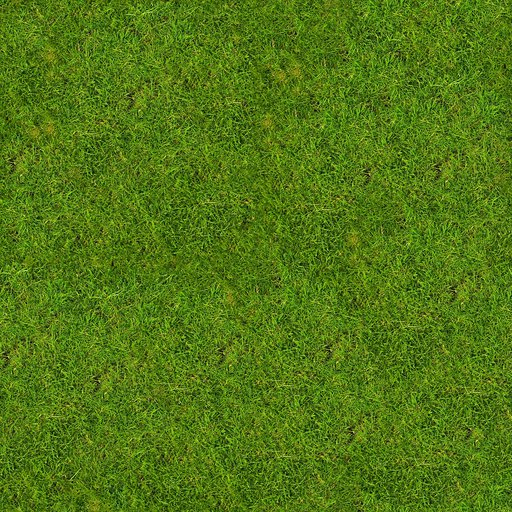
\includegraphics[scale=0.3]{../images/grasslight-small.jpg}
\end{center}
\caption{Grass texture}
\label{grass1}
\end{figure}

\textit{Sky}
\par
Sky object is a sphere (using \textit{SphereGeometry}) \textit{Mesh} object of size 10000 that is surrounding ground plane. Material of this sphere is a texture of blue sky showed on Figure \ref{sky1}. To apply material on internal side of the mesh material's parameter side must be set to \textit{THREE.BackSide}. Full listing of the function \textit{getSky} is showed on the Listing \ref{lst:getsky}.
\\
\lstinputlisting[language=Java,
%commentstyle=\color{green},
firstline=49, lastline=64,
%keywordstyle=\color{blue},
caption={getSky function},
label={lst:getsky}
]
{../js/items.js}

\begin{figure}[h!]
\begin{center}

\includegraphics[scale=1.0]{../images/sky.jpg}
\end{center}
\caption{Sky texture}
\label{sky1}
\end{figure}

\textit{Hay block}
\par
Hay blocks are a constant size 1x1x2 cubits \textit{Mesh} with \textit{BoxGeometry} and hay textured material (Figure \ref{hay1}).

\begin{figure}[h!]
\begin{center}
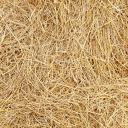
\includegraphics[scale=1.0]{../images/hay.jpg}
\end{center}
\caption{Hay texture}
\label{hay1}
\end{figure}

\textit{Obstacle}
\par
Obstacles are a various size cubits \textit{Mesh} with \textit{BoxGeometry} and rock textured material showed on Figure \ref{obst1}.

\begin{figure}[h!]
\begin{center}
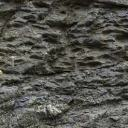
\includegraphics[scale=1.0]{../images/rock.jpg}
\end{center}
\caption{Sky texture}
\label{obst1}
\end{figure}

\subsubsection{utils.js}
Consist of utility functions that are not depend of the logic and structure of the game.
\subsection{Distribution}
Final source code of the project is public accessible as git repository on the GitHub web service by \url{https://github.com/MarcoSchaerfCourses/sino/} link. It could be run online using link \url{https://marcoschaerfcourses.github.io/sino/} since repository was deployed using GitHub Web Pages service.
\newpage
\section{Known Issues}
Testing of final product showed following issues that require additional time to investigation:
\begin{itemize}
\item Performance issues
\item Texture import
\item Bounding Box size increasing depending on rotation of object
\item Adaptation for small screen sizes
\end{itemize}

\newpage
\section{Possible Improvements}
\subsection{Performance}
\subsection{Interface}


\newpage
\bibliographystyle{plain}
\bibliography{biblist}



\end{document}
